\chapter{Introduction}

Humans depend on their vision for every waking hour of the day. Out of the five main senses, vision is arguably the most important in acquring information about the surrounding environment. A person cannot walk in the streets, drive a car, or read if he or she cannot see. However, genetic inheritance, disease, and age will naturally lead to the loss of vision. According to the Vision Council, roughly 75 percent of all adults in the United States require some form of vision correction \cite{GlassesCrafter.com:2010:Vision}. 

The most common method for correcting eye aberrations are with glasses and contact lenses. Both seek to divert the light rays right before they reach the cornea so that the image displayed on the retina, or sensor of the eye, is clear. However, glasses and contact lenses may present an inconvenience. For example, a person who is far-sighted might only need his or her glasses when reading a screen close to him or her and would prefer to not always put on and take off his or her glasses. But what if instead of fixing the eye, the image is modified on the screen so that it appears clear without eyewear? Professor Brian A. Barsky has been focusing on this field for over a decade and introduces to the concept of the vision correcting display in his paper \textit{An Overview of Vision Realistic Rendering and Vision Correcting Displays} \cite{SDTP:SDTP10326}:

\begin{displayquote}
The concept of a vision correcting display involves digitally modifying the content of a display using measurements of the optical aberrations of the viewer's eye so that the display can be seen in sharp focus by the user without requiring the use of eyeglasses or contact lenses. Given the measurements of the optical aberrations of a users eye, a vision correcting display will present a transformed image that when viewed by this individual will appear in sharp focus. Vision correction could be provided in some cases where spectacles are ineffective.
\end{displayquote}


\begin{figure}[ht]
  \centering
  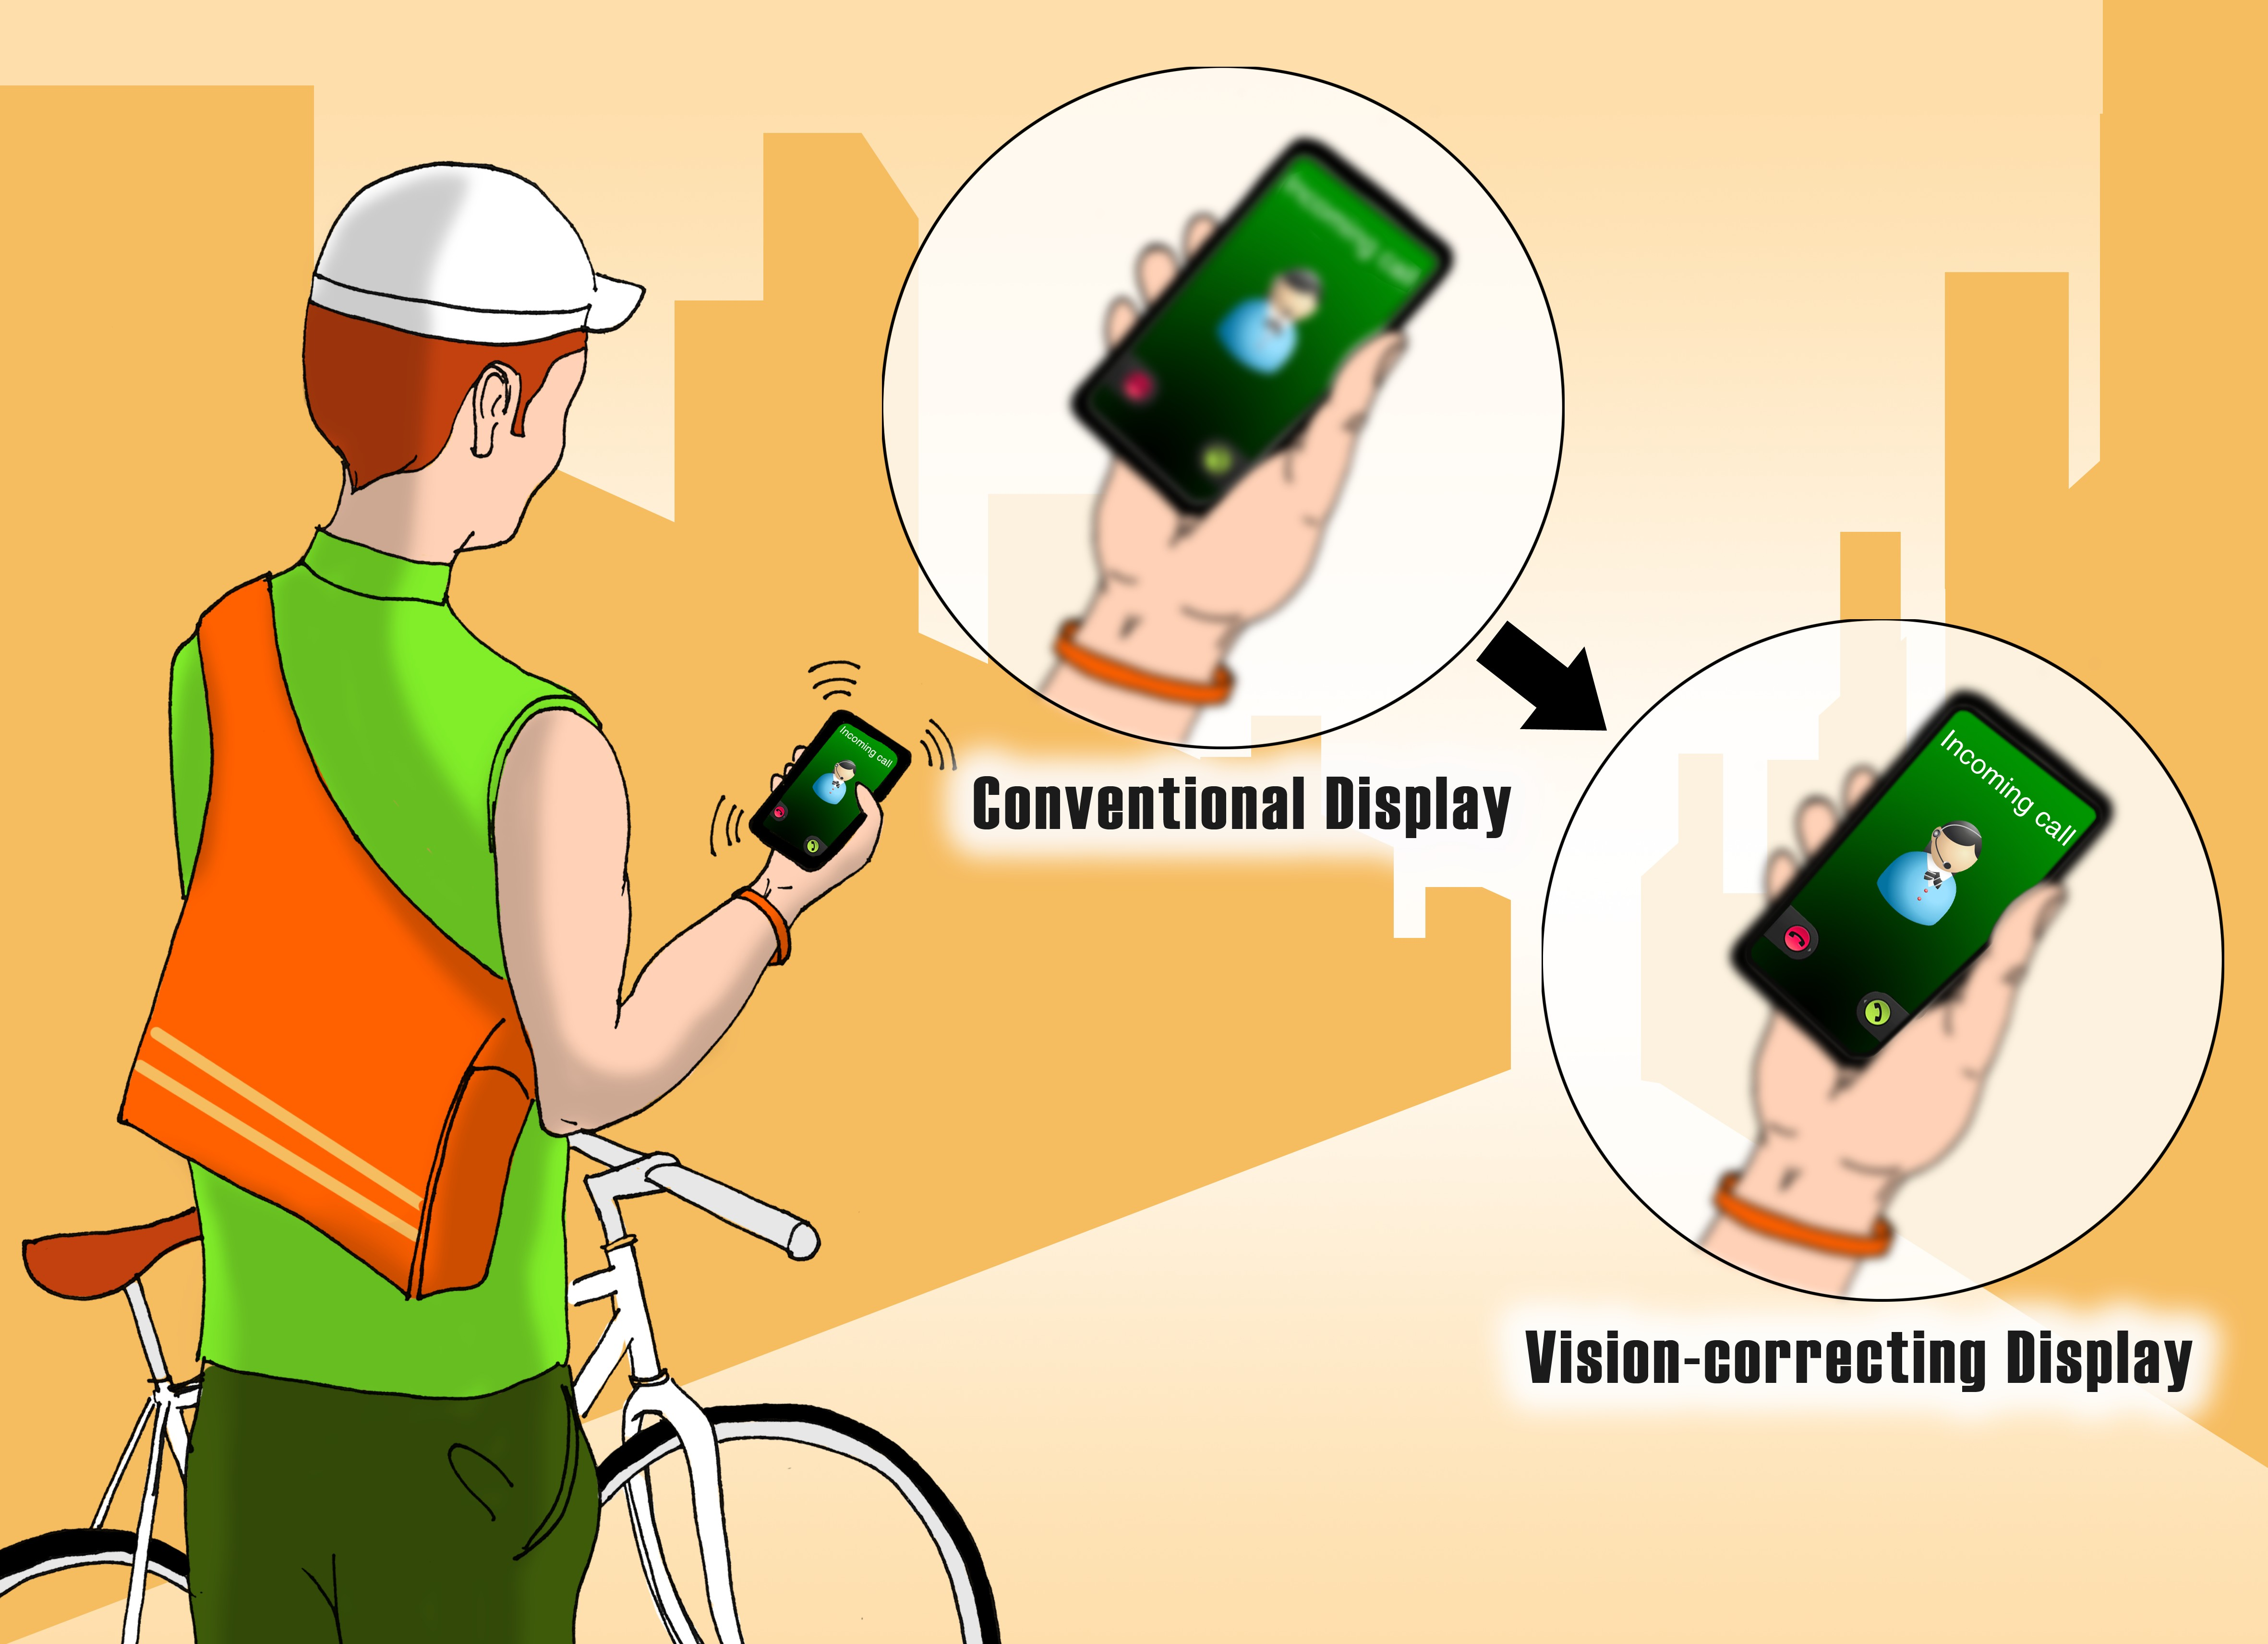
\includegraphics[height=3in]{chapters/chapter1/images/phone.jpg}
  \caption{Application Scenario of Vision-Correcting Display \cite{Huang:2014:VisionCorrectingDisplay}}
  \label{fig:application}
\end{figure}

Fu-Chung Huang et. al proposed two different solutions to this problem. In his first solution, he uses a multilayer display \cite{Huang:2012:COA:2366145.2366204} and in the second one he uses light field technology to generate a sharp image out of the display plane \cite{Huang:2014:VisionCorrectingDisplay}. Wu \cite{Wu:EECS-2016-67} presented one new software algorithm (forward method), one major hardware improvement (lens array display), and a simulation program. 

The goal of this paper is to build on the work from Wu's report. In chapter 4, we present the backward method, which aims to fix some of the issues with the issues with Huang's algorithm. In chapter 7, we test the forward method on different RGB pixel arrangements for different phone screens. In chapter 8, we apply a combined ray and wave optics model in the simulation to account for diffraction and find the optimal size of a pinhole.

% TODO: Finish Reading literature on Huang's algorithm and incorporate it here

%The Chapter 2 of this paper discusses the different types of aberrations of the eye that we aim to correct. Chapters 3 and 4 describe the hardware and software components of the vision-correction display, respectively. Chapter 5 shows the performance of the vision-correction display via physical experiment. Chapter 6 describes the algorithm used for the software simulation of aberrations. Chapter 7 examines the effectiveness of the algorithms on different pixel arrangements of different devices. Chapter 8 is a case study on the effects on diffraction on the effectiveness of the display. Chapter 9 gives a summary of the results of the algorithms presented.